\documentclass{article}

\usepackage{listings}
\usepackage{color}
\usepackage{fancyhdr}
\usepackage{graphicx}

\lstset{language=C,
  commentstyle=\color{red},
  keywordstyle=\color{blue}}

\lstset{ % general style for listings
   numbers=left
   , tabsize=2
   , frame=single
   , breaklines=true
   , basicstyle=\ttfamily
   , numberstyle=\tiny\ttfamily
   , language=C
   , commentstyle=\color{red}
   , keywordstyle=\color{blue}
   , framexleftmargin=13mm
   , xleftmargin=12mm
   %, frameround={tttt}
   , captionpos=b
}
\lstdefinestyle{xslt}
{
    emph={xsl,template,variable,param,for,each,apply,templates,with,param}
    , emphstyle=\color{magenta}
    , emph={[2]match, select, name, mode}
    , emphstyle={[2]\color{cyan}}
}


\begin{document}

\pagestyle{fancy}

\lfoot{\'Equipe 7381} 
\rfoot{Projet C - Semestre 5} 
\lhead{}
\rhead{}

\title{Rapport Projet C - Semestre 5}
\author{DUCOS Joris, DOULIERY Baudouin 
\and Bordeaux INP ENSEIRB}
\date{13 D\'ecembre 2019}
\maketitle
\begin{center}
  \centering
  \huge
  \textbf{Atomic Teddy Investors} \\
  
\includegraphics[scale=0.1]{Logo_INPB.png}
  \end{center}



\newpage
\newpage

\begin{figure}[t]
  \centering
  
\includegraphics[scale=0.5]{teddy.png}
\end{figure}


\newpage

\tableofcontents

\newpage


\section{Introduction}
Ce rapport a pour objectif de pr\'esenter et d'expliquer le travail r\'ealis\'e sur le premier projet de programmation, en premi\`ere ann\'ee \`a l'ENSEIRB-MATMECA.
Le projet porte sur l'impl\'ementation d'un jeu, Atomic Teddy Investors, en langage C. On r\'ealise dans un premier temps une version de base, puis un ensemble d'achievement.\\

Le but principal du projet est d'impl\'ementer le jeu, en langage C. Le probl\`eme principal est donc de d\'efinir un ordre de jeu puis de faire r\'ealiser \`a chaque joueur un nombre de transaction. On peut ainsi se demander comment les diff\'erents \'elements du jeu  vont \^etre mod\'elis\'es ?
Comment la boucle de jeu va fonctionner ? Comment les r\`egles du jeu vont \^etre respect\'ees ?
Tout ces probl\`emes vont \^etre divis\'es en sous-probl\`emes, afin de faciliter le travail. 

\section{R\'esum\'e}
Le projet porte sur le jeu Atomic Teddy Investors.\\

Extrait de \textcolor{red}{\textit{Atomic Teddy Investors :}}\\ 
\textit{"La Sicile a \'et\'e finalement envahie, et les ours ont vaincu l'arm\'ee du Grand-Duc. Se m\^elant aux humains, ils se m\^elent aux divers aspects de la soci\'et\'e, 
reprenant \`a leur compte les divers m\'etiers propres \`a la race humaine. L'un des aspects qui les fascine est celui de l'\'economie de march\'e. Sur les places de 
march\'e de l'\^ile, ils se mettent \`a jouer les magnats, les barons, les grands seigneurs, afin d'arrondir leur p\'ecule personnel ventripotent. Dans leurs costumes 
impeccables, ils prospectent les villes \`a la recherche d'opportunit\'es d'achat et de revente, dans un but finalement assez simple : du miel, rien que du miel. 
Leur app\^at du gain est certainement plus gourmand que cupide, et on admettra que leur compr\'ehension de la m\'ecanique \'economique reste un peu hasardeuse, ce qui 
donne l'objet de ce sujet, qui d\'ecrit ces ensembles d'\'echanges \`a la mani\`ere d'un jeu."}\\

Ce rapport va reprendre la m\'ethode, et les outils qui ont \'et\'e utilis\'es au cours de ce projet.
Il explique alors la d\'emarche employ\'ee, et les choix qui ont \'et\'e fait. 

\vspace*{25mm}

\section{Organisation}

\subsection{R\'epartition des t\^aches}
Pour traiter au mieux le projet, il a \'et\'e divis\'e en plusieurs sous-probl\`emes.
Chaque membre travaille ainsi sur des sous-probl\`emes diff\'erents, afin d'avancer le plus vite possible.
La r\'epartition des t\^aches c'est faite de mani\`ere assez intuitive, sans trop de probl\`eme pour organiser le travail au sein le bin\^ome. 
Afin de pouvoir travailler en simultan\'e, et pour s'\'echanger des fichiers facilement, un syst\`eme de d\'ep\^ot a \'et\'e mis en place. 

\subsection{Outils utilis\'es}

\subsubsection{D\'ep\^ot (forge)}

Le partage des fichiers c'est fait en utilisant le syt\`eme de d\^epot Thor, mis en place par nos professeurs encadrants. 
L'utilisation de git a permis d'envoyer les fichiers sur le d\^epot Thor, et ainsi d'\'echanger les informations entre co\'equipiers.
Le d\^epot permet aussi de faire passer des test \`a nos fichiers, et ainsi de verifier que tout fonctionne correctement. 
 

\subsubsection{\LaTeX}

Ce rapport est r\'edig\'e en \LaTeX. Les fichiers relatifs \`a son \'ecriture sont pr\'esents sur le d\'ep\^ot. 

\subsubsection{Makefile}
Dans le but de faciliter et de controler l'\'etape de compilation, nous utilisons un ficher Makefile, qui suit le principe de fonctionnement ci-dessous :
\begin{figure}[h]
  \begin{center}
  \fbox{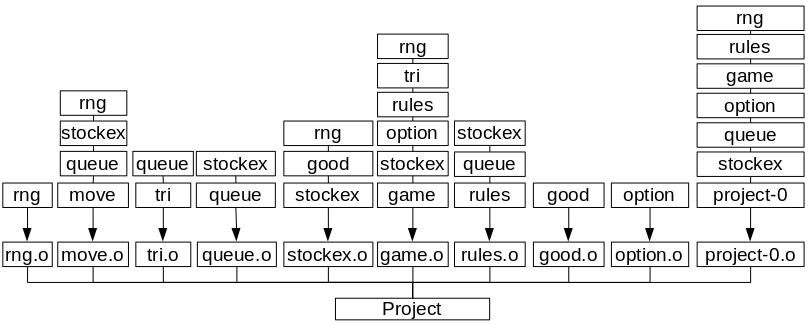
\includegraphics[scale=0.4]{Makefile.png}}
  \caption[le titre]{Makefile et D\'ependance}
\end{center}
\end{figure}

%\vspace*{50mm}

\section{Mise en place de l'algorithme}

\subsection{Principe de la boucle de jeu}

\`A partir des consignes, et des explications de l'\'enonc\'e, nous avons pu mettre en place un algorithme pour la boucle de jeu. 
Le principe est de faire tourner la partie durant un temps pr\'ed\'efini, tout en assurant le respect des r\`egles.
Au lancement de l'executable, il est possible de choisir certaines conditions, comme le nombre de joueurs, ou bien le nombre de tours.\\

Pendant un tour de la partie, la premi\`ere \'etape est de selectionner le joueur prioritaire, c'est \`a dire le joueur avec le temps de jeu le plus
faible. Donc une file de priorit\'e doit \^etre mise en place. 
Ensuite il faut le faire choisir une transaction parmis celles propos\'ees par la place d'\'echange (au d\'ebut du projet, il n'y avait qu'une seule place
d'\'echange) de mani\`ere al\'eatoire, puis ensuite il va r\'ealiser cette transaction un nombre de fois al\'eatoire entre \textbf{0 et 10}.
Une fonction qui permet d'avoir un nombre al\'eatoire entre ces bornes est alors impl\'ement\'ee. 
Une fois la transaction r\'ealis\'ee, le joueur est sorti de la file, et replac\'e \`a la fin. Ce joueur ne jouera pas au tour suivant.\\

Au cours du projet, plusieurs places d'\'echanges ont \'et\'e implant\'ees, ce qui apporte en plus la notion de d\'ecision pour les teddies.
Elles sont accessible ou non en fonction de la transaction choisie. 
Les joueurs doivent visiter toutes les places d'\'echanges, donc la code doit tenir compte de celles visit\'ees avant.\\

\`A chaque tour, les joueurs doivent respecter les r\`egles, sinon ils sont exclus. Autrement dit, si le teddy "choisit" un nombre de transactions sup\`erieur \`a ce que permet son portefeuille, la fonction \textit{kick or keep} se charge de l'\'ecarter du jeu. 
Apr\`es le dernier tour du jeu, les r\'esultats des joueurs restants sont r\'ecup\'er\'es, les joueurs sont class\'es, et le classement est affich\'e. 


\subsection{Cr\'eation des structures et variables globales}

\subsubsection{Les constantes}

\begin{itemize}

\item Le premier type de constantes mis en place sont les constantes qui vont \^etre utilis\'ees au cours du jeu, comme par exemple les differentes ressources,
qui sont d\'efinies dans le fichier \textbf{good.h}, ou bien comme les diff\'erentes places d'\'echanges, d\'efinies dans \textbf{stockex.h}.
\item Les autres constantes d\'efinies sont les constantes relatives aux r\`egles et limites du jeu, comme le nombre maximal de tours, de joueurs, ou bien de ressources. 
Ces constantes pourront \^etre entr\'ees comme argument lors de l'appel de l'executable, et ainsi les parties seront personnalisables. 

\end{itemize} 

\vspace*{10mm}

\subsubsection{Les structures}

\begin{itemize}

\item\textbf{Wallet}

La structure "Wallet" est la structure qui correspond au portefeuille d'un joueur.
Elle est compos\'ee d'un tableau d'entiers, qui correspondent aux quantit\'es de chaque ressources que le joueur poss\`ede.


\begin{lstlisting}[style=xslt]
// A wallet containing different amounts of goods
struct wallet 
{
  unsigned int data[MAX_GOOD];
};
\end{lstlisting}

\item\textbf{Stockex}

La structure "Stockex" est la structure qui correspond \`a une place d'\'echange.
Elle est compos\'ee d'une chaine de caract\`eres, qui donne le nom de la place d'\'echange, d'un entier indiquant le nombre de transactions r\'ealisables dans cette place d'
\'echange,
et enfin d'un tableau de transactions.
Elle est construite de la m\^eme mani\`ere que la structure Wallet.

\item\textbf{Transac}

La structure "Transac" est la structure qui correspond \`a une transaction.
Elle est compos\'ee de deux portefeuilles, qui correspondent respectivement aux ressources vendues par la place d'\'echange, et \`a celles achet\'ees par cette m\^eme place d'\'echange.
Au cours du projet, l'identifiant du stockex auquel appartient la transaction est rajouté \`a la structure, ainsi que l'identifiant du stockex auquel elle m\`ene. 
Elle est construite de la m\^eme mani\`ere que la structure Wallet.

\item\textbf{Queue}

La structure "Queue" est la structure qui correspond \`a la file de joueurs.
Elle est compos\'ee d'une liste de pointeurs vers des joueurs, ainsi que du nombre de joueurs pr\'esents dans la file. 
Elle est construite de la m\^eme mani\`ere que la structure Wallet.

\item\textbf{Teddy}

La structure "Teddy" est la structure qui correspond \`a un joueur.
Elle est compos\'ee d'un portefeuille, d'un num\'ero d'identifiant, d'un temps de jeu, d'un nombre de ressource \'equivalent en "Honey".
Durant le d\'eveleppoment de l'achievement 1, nous avons ajout\'e le nombre de places d'\'echanges visit\'ees, la liste avec ces places d'\'echanges, et enfin la localisation actuelle du teddy.
Elle est construite de la m\^eme mani\`ere que la structure Wallet.

\end{itemize}

\vspace*{10mm}

\subsection{Impl\'ementation d'une file de priorit\'e}
Apr\`es la cr\'eation des structures et des variables globales, il faut mettre en place la file de priorit\'e, dans les fichiers \textbf{queue.[ch]}. Les teddies int\'eragissent avec les places d'\'echanges en suivant un ordre de priorit\'e. La r\`egle dit que le teddy prioritaire est celui avec le temps de jeu le plus faible.\\ 
Donc la structure correspondante \`a un teddy comprend un portefeuille, un num\'ero d'identification, et un temps de jeu.\\ 

La solution choisit pour mod\'eliser la file est une liste de pointeur vers des teddies, ainsi qu'un entier indiquant le nombre de teddies dans la file. 
Les fonctions cod\'ees permettent de cr\'eer une file, ou bien d'int\'eragir avec la file, en faisant entrer un teddy, ou en faisant sortir le teddy prioritaire, et ainsi pouvoir le faire jouer. 
C'est aussi dans ce fichier qu'est d\'efinie le nombre maximal de joueurs.\\

Les premiers probl\`emes rencontr\'es \'etaient li\'es \`a l'initialisation des teddies. Finalement, le code initialise les teddies un par un, et cr\'ee un tableau de pointeur vers ces derniers.
Ensuite, l'autre probl\`eme concerne la file et le classement des teddies dedans.
La solution adopt\'ee est de ne s\'electionner que le teddy prioritaire, et de ne pas appliquer de classement sur le reste de la file. Le d\'efaut de cette m\'ethode est que la recherche du teddy prioritaire doit se faire \`a chaque tour.  


\subsection{Impl\'ementation des fichiers}

\begin{itemize}

\item\textbf{good.[ch] :} Les premiers fichiers mis en place sont les fichiers good.[ch].\\
Les fichiers good vont d\'efinir les differentes ressources que peut acheter ou vendre un teddy, mais aussi la structure du portefeuille, le "wallet". 
\`A chaque ressource est associ\'ee une valeur.
C'est dans ce fichier qu'est d\'efinie la valeur maximale de ressources differentes.
Aucun probl\`eme n'a \'et\'e rencontr\'e pour coder good.[ch], mais il se peut que plus tard dans le projet il y ait des conflits, \`a cause de certaines modifications de types. 

\item\textbf{stockex.[ch] :}  Les fichiers suivants ont \'et\'e les fichiers \textbf{stockex.[ch]}, qui impl\'ementent la notion de place d'\'echange, appell\'ees ici "stockex".\\
Une place d'\'echange va \^etre carat\'eris\'ee par une structure, contenant un nom,un nombre de transactions, et les transactions. 
Chaque transaction est d\'efinie par une portefeuille entrant, et un protefeuille sortant, aussi mod\'elis\'ee par une structure.
C'est dans ce fichier qu'est d\'efinie la valeur maximale de transactions differentes par place d'\'echange.\\
Lors de la mise en place des places d'\'echanges, les probl\`emes rencontr\'es sont principalement dus \`a l'\'ecriture des pointeurs, mais ils ont vite \'et\'e surmont\'es.

%Pour le moment, une seule place d'\'echange est utilis\'ee, elle est d\'efinie dans le fichier stockex.h, d'apr\`es l'exemple de l'\'enonc\'e mais il serait pertinent de co%der une fonction qui permet de g\'en\'erer un stockex, avec des caract\'eristiques al\'eatoire.

\vspace*{10mm}

\item\textbf{queue.[ch] :} La file de priorit\'e est g\'er\'ee dans les fichiers \textbf{queue.[ch]}.\\
C'est \`a ce moment que la structure de la file est cr\'e\'ee.
Un ensemble de fonctions sont d\'efinies, afin de faire fonctionner la file, donc il y a une fonction qui d\'efinit le joueur prioritaire, une autre qui le selectionne,
et le fait sortir de la file.
Ces fichiers sont li\'es avec \textbf{stockex.[ch]}, car ils utilisent les carat\'eristiques des teddies pour faire \'evoluer la file.

\item\textbf{game.[ch] :} Ces fichiers vont rassembler l'ensemble des diff\'erents codes, pour pouvoir mettre en place les focntions qui vont faire fonctionner le jeu,
comme par exemple la fonction \textit{play}.
Cette fonction est la plus importante de l'executable.  

\item\textbf{rules.[ch] :} Le jeu est r\'egi par certaines r\`egles, qui vont \^etre d\'efinies dans les fichiers \textbf{rules.[ch]}.\\
Les fonctions v\'erifient que les r\`egles sont respect\'ees. Une autre fonction  va indiquer si le teddy doit \^etre exclue ou non.\\
Ces fonctions sont utilis\'ees dans la boucle de jeu finale. 

\item\textbf{move.[ch] :} L'achievement 1 a offert aux teddies la possibilit\'e de changer de stockex. Afin de pouvoir r\'ealiser ce mouvement, des fonctions ont \'et\'e \'ecrites dans \textbf{move.[ch]}.\\
Elles prennent en compte la position actuelle du teddy, et les postions auxquelles il peut se rendre, en fonction des transactions \`a sa disposition. 

\item\textbf{rng.[ch] :} Ces fichiers impl\'ementent simplement la fonction de g\'en\'eration de nombre al\'eatoire, qui sera utilis\'ee dans le projet. 

\end{itemize}

\subsection{Affichage des r\'esultats}

Une fois la partie termin\'ee, c'est \`a dire une fois que chaque teddy a un temps de jeu \'egal au temps de jeu maximal d\'efini en d\'ebut de partie, il faut afficher les r\'esultats.
Ainsi, la fonction 
\textit{display results} 
se charge d'afficher le classement.
Pour chaque teddy restant, elle calcule l'\'equivalent-Honey de son 
\textbf{wallet},
puis elle effectue un 
\textbf{tri par insertion} 
sur la file de priorit\'e compos\'ee des teddies.\\

Nous avons d\'ecid\'e de choisir ce tri car, m\^eme s'il est d'une complexit\'e asymptotique quadratique, il est en moyenne beaucoup plus rapide que le quicksort ou que tri fusion pour des jeux de donn\'ees de petites tailles.
Or, notre projet s'effectue dans un contexte de 20 teddies maximum. \\
C'est donc pour cette raison que le tri que nous avons choisi d'impl\'ementer est le tri par insertion.

\vspace*{25mm}

\section{Tests r\'ealis\'es}
Afin de v\'erifier le code, un fichier de test est mis en place. 
Les tests r\'ealis\'es permettent de mettre en avant tout les r\'esultats faux, apr\`es l'execution de certaines fonctions. 
Ces tests n'ont \'et\'e r\'ealis\'e que sur certaine fonctions, mais auraient 
pu \^etre effectu\'es sur des fonctions diff\'erentes. 
Ces tests ne servent que \`a aider pour le code, mais ils ne remplacent pas les 
tests impos\'es par la forge de l'\'ecole. 
 

\section{Conclusion}

Ce projet a permis \`a chaque membres du groupe d'am\'eliorer ses comp\'etences en langage C, et en \LaTeX.
La division du projet en sous-probl\`emes nous a appris comment relier diff\'erents fichiers, g\'erer les erreurs, et ainsi pouvoir construire un fichier executable.
De plus, nous avons beaucoup appris sur le travail de groupe, et comment bien g\'erer les partages de fichiers. 
Cependant, le projet n'est pas encore fini, et il reste des achievements \`a traiter. Nous avons fini l'achievement 1, qui consistait \`a implanter dans le 
jeu plusieurs places d'\'echanges, et \`a faire intervenir le choix des teddies. L'achievement 2 leur impl\'ementera la notion de strat\'egie. 
Ainsi, nous avons r\'eussi \`a faire fonctionner le jeu, m\^eme si il y a encore beaucoup de points d'am\'eliorations, et d'\'evolutions possibles sur le projet. \\

\vspace*{10mm}

Sources images :
\begin{itemize}

\item\textit{Représentation enfantine classique du "nounours"} par Fr\'ed\'eric Bellaiche.

\item Logo Bordeaux INP ENSEIRB

\end{itemize}


\end{document}